\chapter{Chatbots}
\label{chap:chatbots}

Based on latest MMC's state of AI report\footnote{The State of AI 2019: Divergence \autocite{report:Kelnar2019}}, it appears that 26\% of the AI-Startups studied by Gartner\footnote{2'791 European AI Startups from the 2019 CIO Survey: CIOs Have Awoken to the Importance of AI \autocite{online:gartner_2019_ai_survey}} are using or making chatbots, see Figure~\ref{fig:fig_mmc_state_of_ai_2019_gartner_cio_survey_31}. The same study, made a year earlier, in 2018, shows that chatbots are not present as an application, which implies that either chatbots were not referenced as AI or that their popularity exploded within a year.\\

As it is at the beginning of 2020, based on The State of AI Report 2019 \autocite{studies:state_of_ai_2019} and the two previously mentioned studies, chatbots are commonly present but limited to narrow tasks. In most cases, they a scenario-based with sequences of if-else conditions that we classify as non-learning \gls{ai}. Moreover, hard-coded scenarios are requiring an infinite amount of human power to create generic Chatbots able to maintain a conversation at a human level. However, progress in the field of \gls{ml} and \gls{nlp} is demonstrating that providing large corpora to an unsupervised algorithm is enough to maintain a passive conversation with users, which results into a shifting of the human power into data engineering. Increasingly complex algorithms and techniques are emerging at a monthly in the field, demonstrating a trend towards conversational performance improvements. Note that even if they are getting better at providing meaningful sentences, current Chatbots are still not able to orchestrate the generalization of all the tasks required to a human-like conversation. E.g., such as understanding and reasoning based on the context, initiatives to search and learn for missing information, initiate dialogue in a meaningful manner, intuition, and much more. As a side note, the generalization of those tasks would reduce the steps significantly towards general Chatbots.\\

From a user-centric point of view, chatbots are currently trending and rising global interest for various reasons. Big companies such as \textit{Google} or \textit{Apple} are believing in the technology and are making a lot of effort at pushing the chatbots into the mainstream. Even if the word \say{chatbot} is commonly used as a buzzword without a proper definition, people have at least a mental representation of its concept. Indeed, whether they call it \say{Digital Assistant}, \say{Siri}, \say{ok Google} or \say{Alexa}, they all expect to a more or less human-like conversations after using those triggering keywords.\\

It is interesting to note that the majority of the following sections could be included in the field of \gls{ai} in general. The extrapolation of the chatbot subject to \gls{ai} as a whole is worth further studying, but it not part of this work. Instead, the focus of this chapter is Chatbots; we provide a synthesis and classification of the different methods used to build chatbots. We will define the main categories identified and continue on the main sub-categories and conclude with a cartographical chart of our chatbot vision.


%\clearpage

\begin{figure}[H]
    \centering
    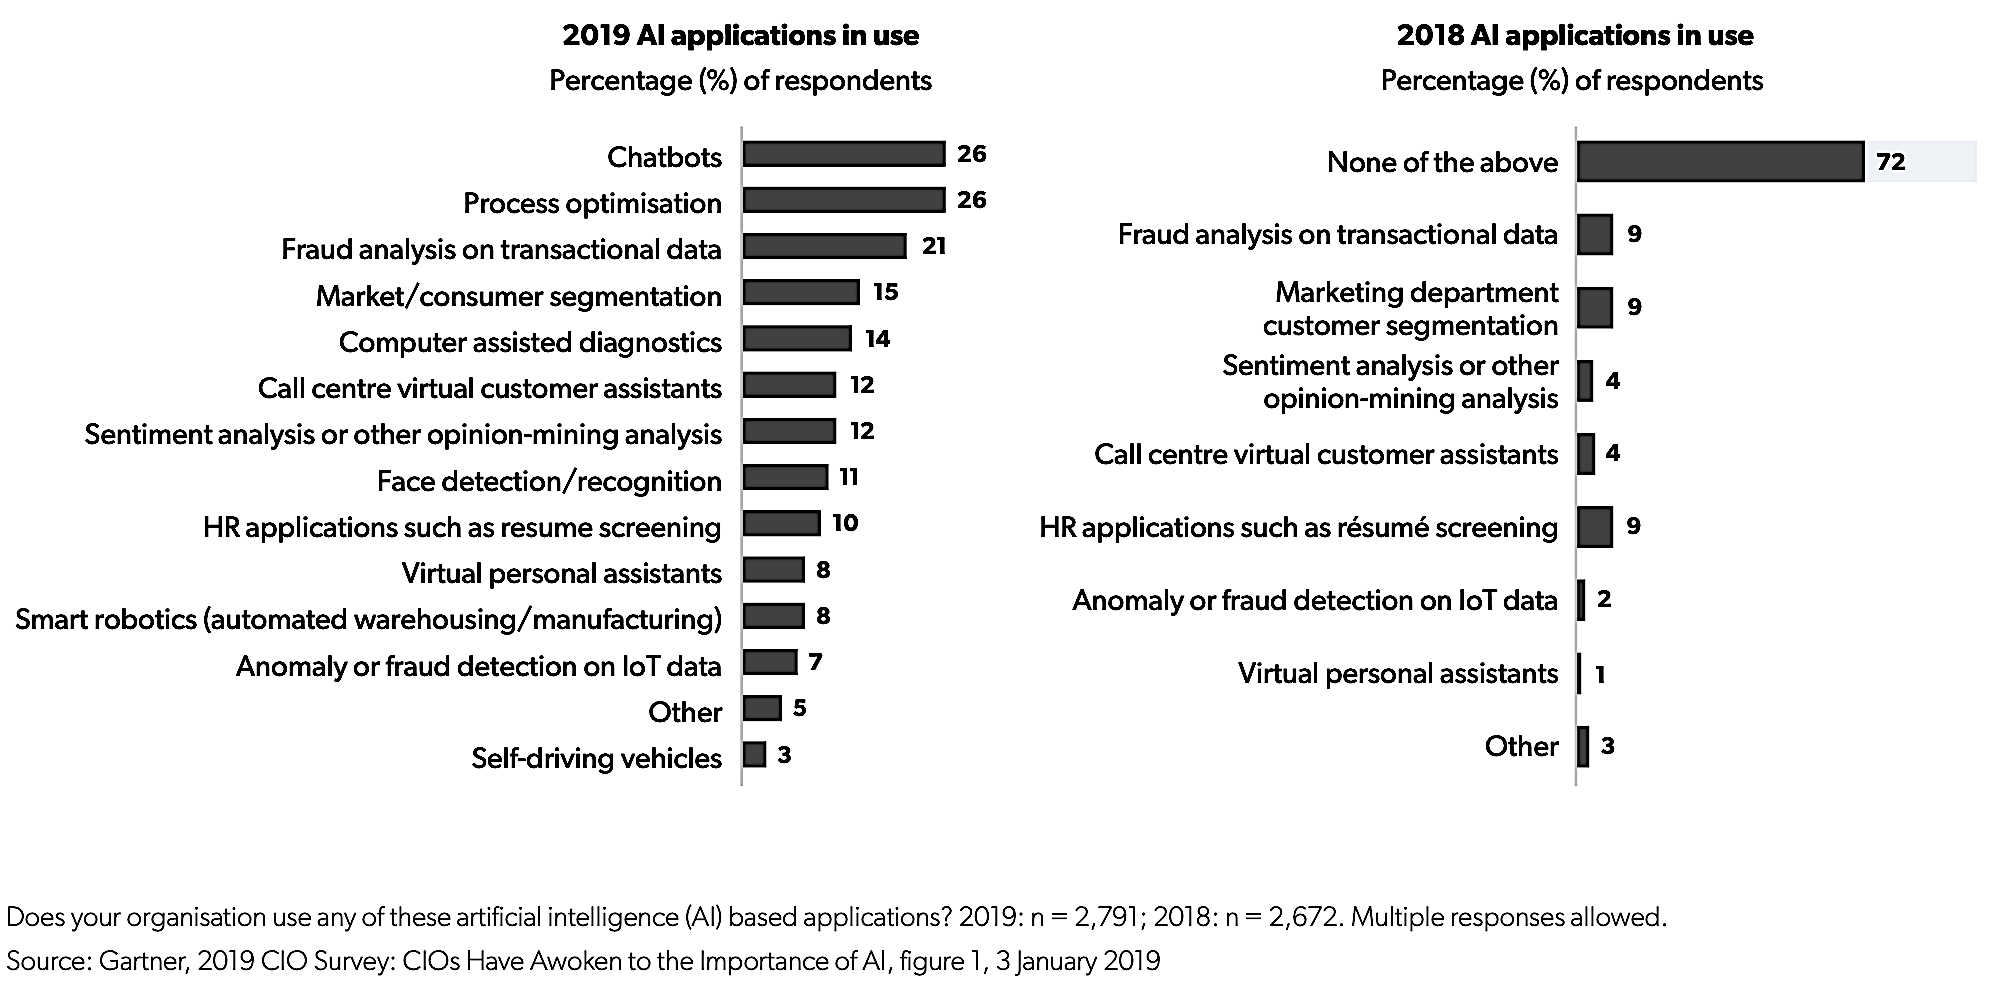
\includegraphics[width=\textwidth,keepaspectratio=true]{fig_mmc_state_of_ai_2019_gartner_cio_survey_31}
    \caption{Figure 31 from \textit{The State of AI 2019: Divergence \autocite{report:Kelnar2019}}. The top \gls{ai} applications used in European AI Startup in 2019 are Chatbots and Process optimization.}
    \label{fig:fig_mmc_state_of_ai_2019_gartner_cio_survey_31}
\end{figure}



\section{Chatbot History}
\label{chatbot:history}
Not mentioning \textit{Alan Turing} or \textit{Joseph Weizenbaum}, both considered as the fathers of \gls{ai} and chatbots, would not be fair to this research. Indeed, in 1950 they forecasted human-like communication with computers and proposed a test to differentiate humans from machines, the Turing Test \autocite{paper:turing}. The test performs as follows: a supervisor asks a human to talk to a masked entity and determine rather he is talking to a human or a computer. If the human cannot recognize speaking to a computer, then the machine passes the Turing test.\\

In 1966,\textit{Joseph Weizenbaum} wrote Eliza\autocite{website:eliza}, a computer program simulating a psychotherapist, it is seen today as one of the first well-documented attempts to make a Chatbot designed at passing the Turing test. However, due to techniqueal restrictions, Eliza was not performing particularly well in all contexts. As for today, it is still possible to play with the chatbot on a dedicated website.\\

Since Eliza, a lot of progress has been made until 2020, From conditional IF-ELSE, \gls{aiml}, up to \gls{ml} with \gls{ann} and \gls{dnn}, the improvements in the field of chatbots increased drastically over the years. Each iterations delivering algorithms being continuously more sophisticated and better at using the \gls{nl}, resulting in a new field of \gls{ml} called \gls{nlp}. As a reminder of the chatbots history and progress from 1966 to 2016, the  infographic\autocite{online:futurism_history_infography} from Futurism is particularly speaking. 


\section{Main Categories in the Chatbot Realm}
\label{chatbot:main-cats}
While performing the state-of-the-art, we identified three main chatbots categories. 

\subsection{Conversational}
We like to call them the Chatty bots, and they are great for interaction and structured replies, well designed for their ability to talk. E.g., \textit{User}: \say{Hello, how are you?}, \textit{Bot}: \say{Good, what about you?}.

\subsection{Task-Oriented}
The Task-Oriented bots are performing particularly well at specific tasks as smart-assistants. As their design is not toward generalization, their abilities are limited and will fail at off-tasks. A common workflow used by those bots is to detect the Intent and the Entities of the user request, often in \gls{nl}, then apply a rule-based matching to perform the command intended by the user. E.g., \textit{User}: \say{Book the next flight to Geneva from Zürich.}, \textit{Bot}: \say{Alright! Your ticket number is 00XXYYZZ. Have a great flight!}

\subsection{Dispatcher}
The dispatcher acts as a middleware, who's unique job is to categories the user input and forward the input to the task executor from any of the previous two categories that the user requested. E.g., If the user request the following "What is the weather in Geneva?", the dispatcher will categories the question as the task of providing the weather and sent it to the weather module. As a second example, if the user provides the following input "Hey! Let's talk about random stuff!", the dispatcher will forward the request to the chatty module.


%\clearpage

\section{Retrieval Chatbots}
\label{chatbot:retrieval}
As it is today, Retrieval-based Chatbots are popular in the industry. Indeed, a lot of tools are available, and they perform well for specific tasks. However, the response capabilities are limited to their databases and the retrieval algorithm used. Indeed, for a given input, the system is using heuristics to find the best output from the pre-defined responses. The choice of the algorithms is wide and depends on the task the chatbot is required to perform. Regardless of the heuristic used, from keywords matching up to \gls{dl}, the output will always be retrieved from the database. Concerning the database itself, the data needs a pre-processing step to generate indexes linking the questions, answers, and apply pre-calculated scores. Pre-processing also implies that if the database is updated, a new pre-processing batch is required, which implies that the scalability or fine-tuning if compromised in the long run. We like to call this type of chatbots \say{Keywords-based}. See Figure ~\ref{fig:fig_retrieval_chatbot}.

\begin{figure}[H]
    \centering
    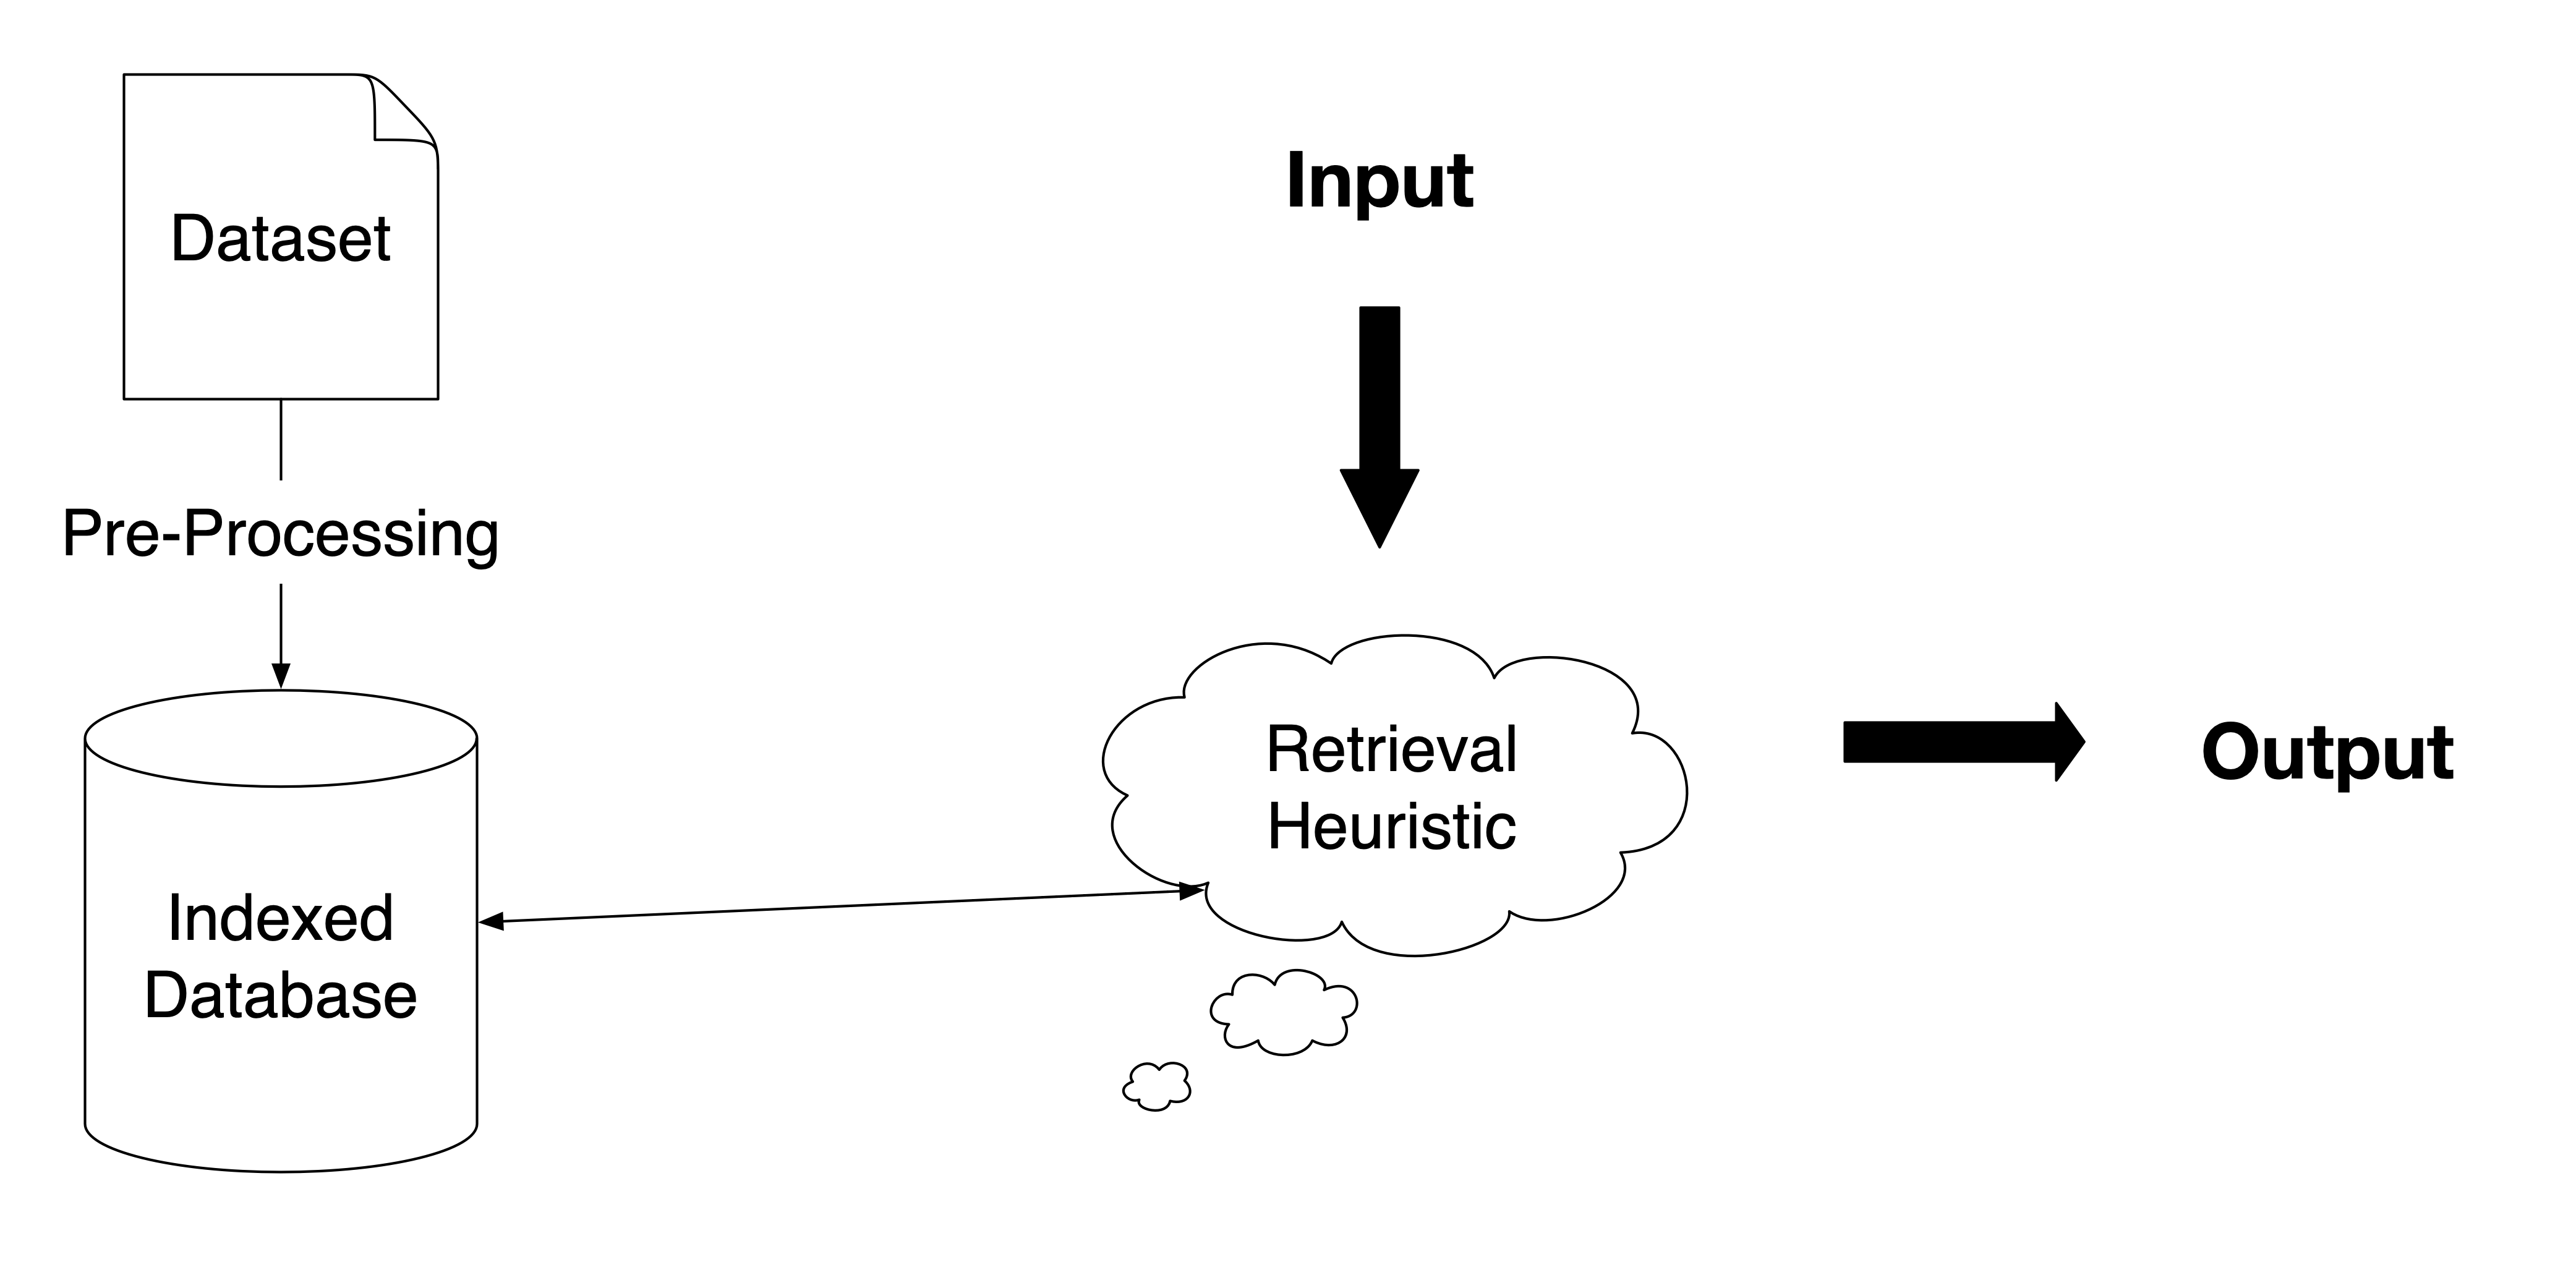
\includegraphics[width=\textwidth,keepaspectratio=true]{fig_retrieval_chatbot}
    \caption{Illustrative representation of frequent retrieval chatbots architecture.}
    \label{fig:fig_retrieval_chatbot}
\end{figure}


\section{Rule-Based Chatbots}
\label{chatbot:rulebased}
\say{Scenario-based}, as we name it, is the oldest and relatively straightforward system for chatbots. The Eliza\cite{website:eliza} Chatbot, as mentioned in the Chatbot History \ref{chatbot:history}, is scanning the input text for keywords, calculates a ranking for each keyword, and finally goes through a series of conditions called rules, and some randomness to reach the best ending leaf. Usually, the bot also includes a default output if the matching process fails, which we can still nowadays see in chatbots: \say{Hmm, this is interesting, tell me more.}. Such bots are often used for interactive chatbots, as it can, in a controlled environment, give a sense of deep meaning in the context of the conversation. Note that such systems require a lot of human power to build a frame for the bot to play in, and by this mean makes rule-based chatbots great for the specific scenario but is hard particularly hard to generalize. See Figure ~\ref{fig:fig_rulebased_chatbot}.

\begin{figure}[H]
    \centering
    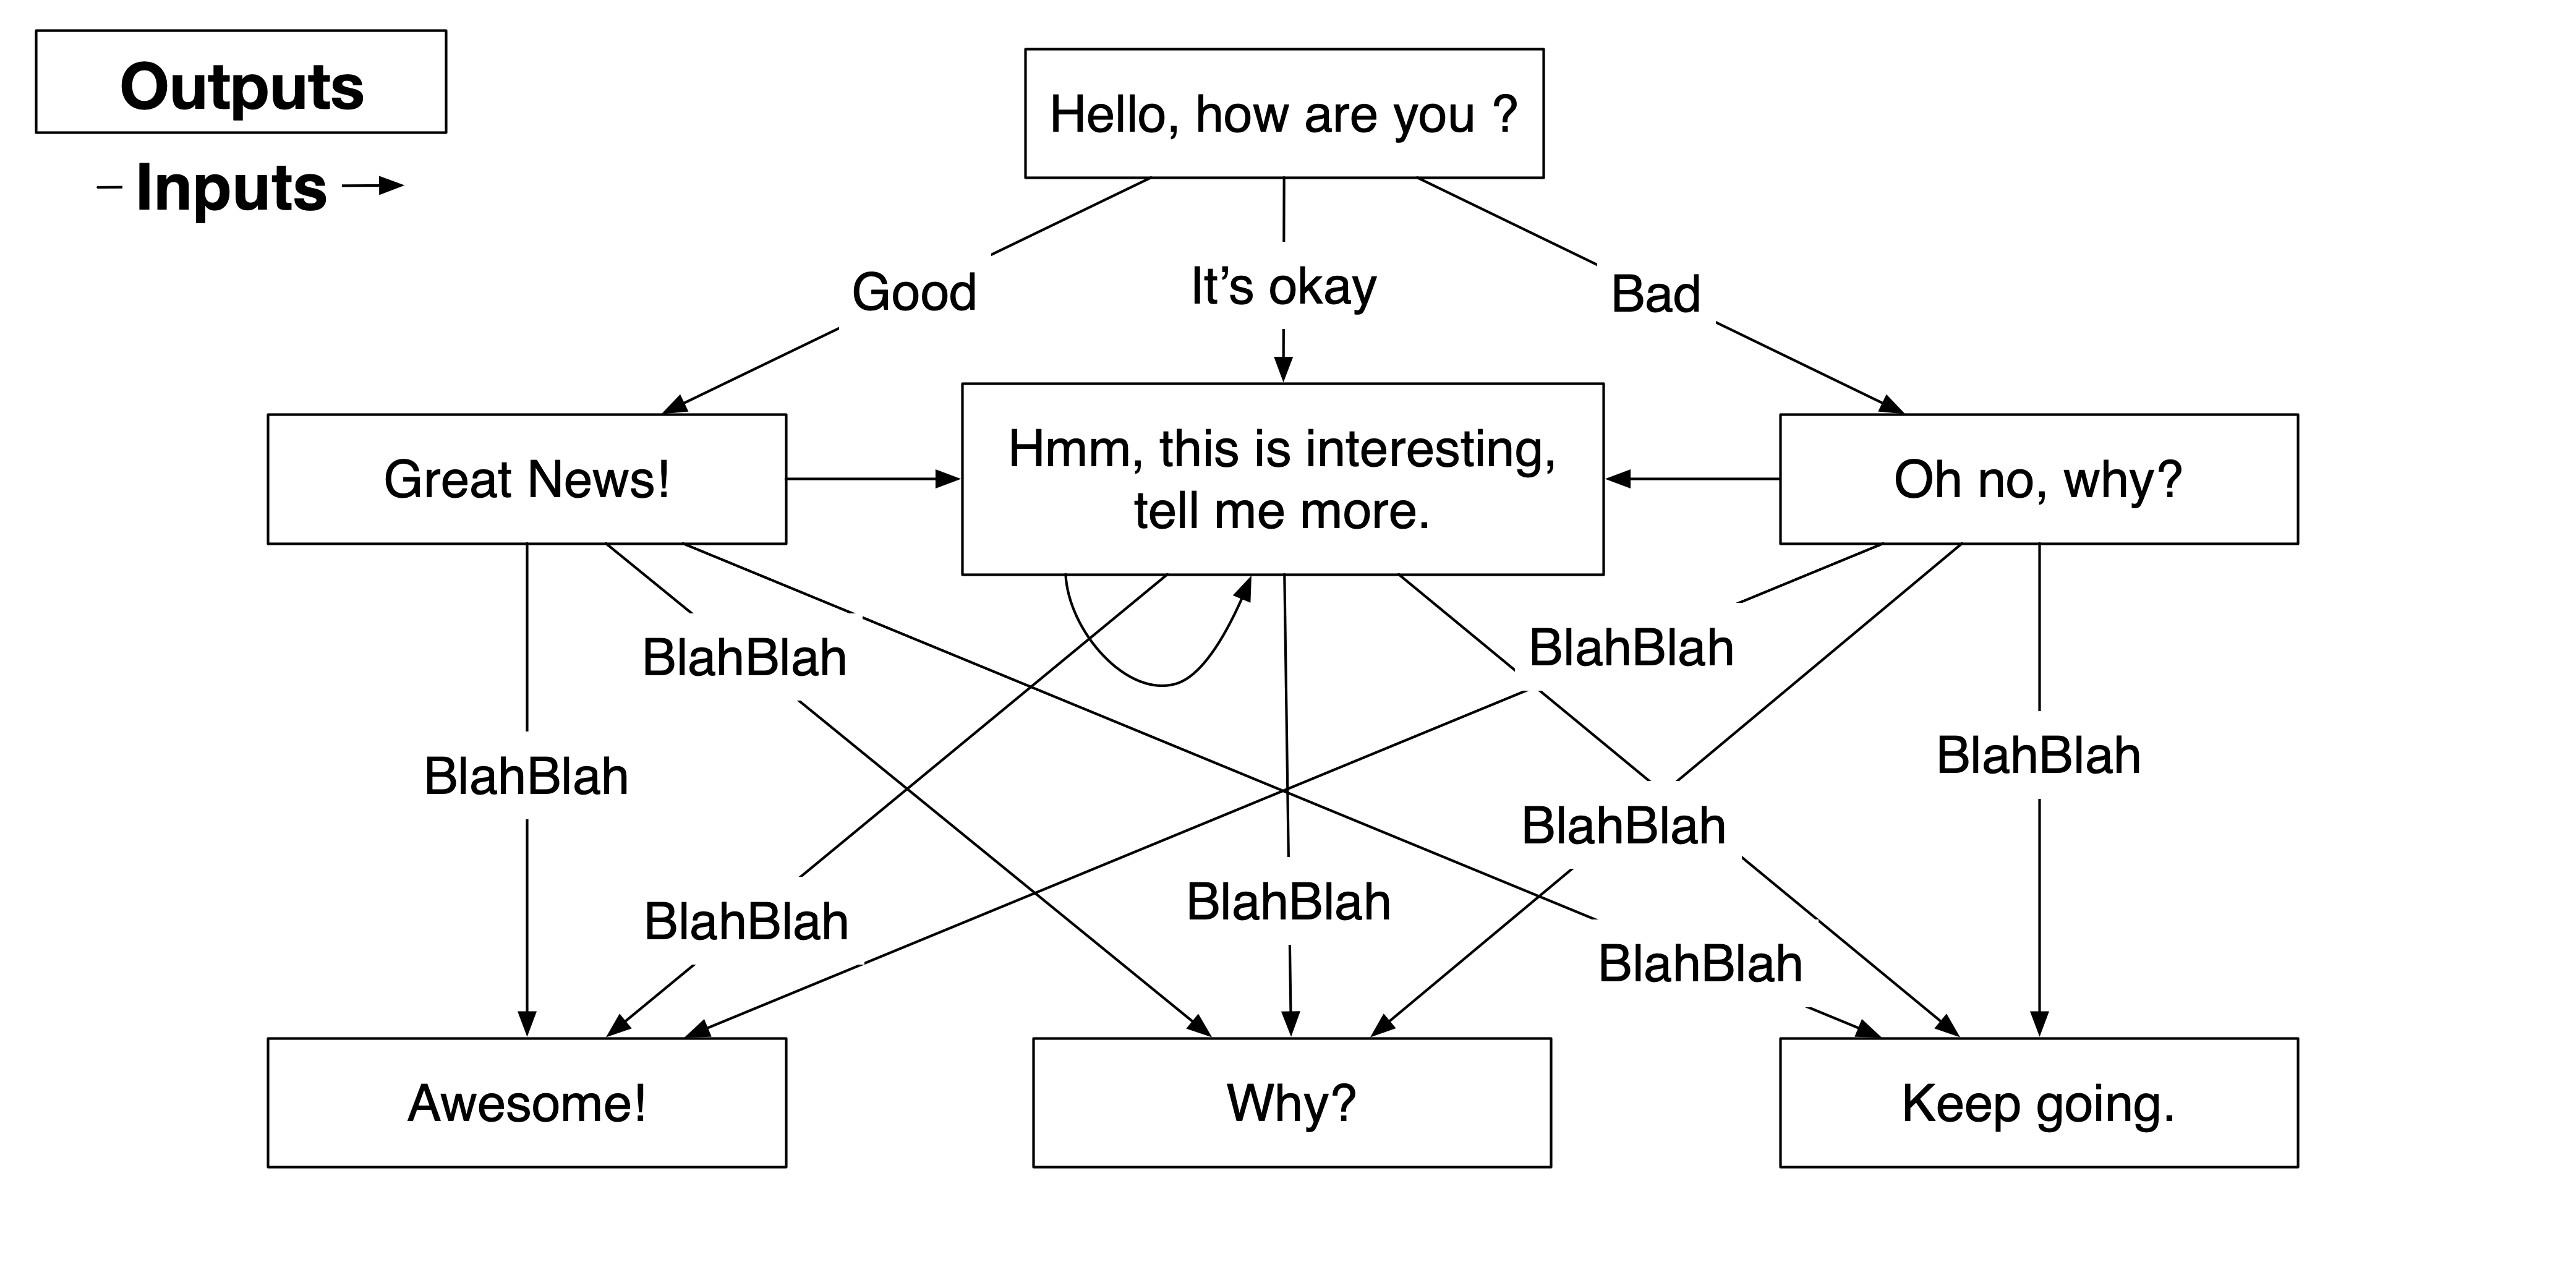
\includegraphics[width=\textwidth,keepaspectratio=true]{fig_rulebased_chatbot}
    \caption{Illustrative representation of frequent rule-based chatbots process.}
    \label{fig:fig_rulebased_chatbot}
\end{figure}

\section{Generative Chatbots}
\label{chatbot:generative}
As the current result of all the incredible innovations made in the past years in \gls{nlp}, and is a premise to true conversational chatbots, generative methods are overcoming the limitations of the Retrieval \ref{chatbot:retrieval} and Rule-Based \ref{chatbot:rulebased} Chatbots, by its ability to generate new content. Either Supervised \ref{chatbot:supervised}, Unsupervised \gls{ul} or Adversarial \ref{chatbot:adversarial}, no pre-defined outputs are used, the models are trained on large corpora to learn the language patterns and outputs relatively meaningful responses to give inputs. Another particularity of generative chatbots, is that building a domain-oriented chatbot does not require the engineers to have the domain expertise, as the expertise is embedded into the data, which allows a relative scalability to new domains. However, even if the trained models can output responses at nearly no timespan, the data-engineering of the datasets and the training phase is most often long and complicated. As a final note, the responses generated by such chatbots are only as good as the data it was fed during the training.

\subsection{Supervised Learning}
\label{chatbot:supervised}
\gls{sl} is probably the most common method used by Generative Chatbots, as it provides relative control over training. \gls{seq2seq} is commonly used as architecture for those chatbots, a \gls{nlp} version of the \gls{enc-dec}, which encodes the input words sequence and decode it into a words sequence as an answer into a framed conversation fashion. The training only requires a dataset containing a sentence and its desired response, the model will then map similar inputs with similar outputs. However, a clear limitation for this learning is that the model will for any input always have an answer, regardless of the overall meaning. Additionally, \gls{seq2seq} will prioritize the highest word apparition probabilities, meaning that data duplicates and requiring sentences will create a trend during decoding. E.g., \say{I don't know the answer.}. See Figure ~\ref{fig:fig_supervised_chabots} 

\begin{figure}[H]
    \centering
    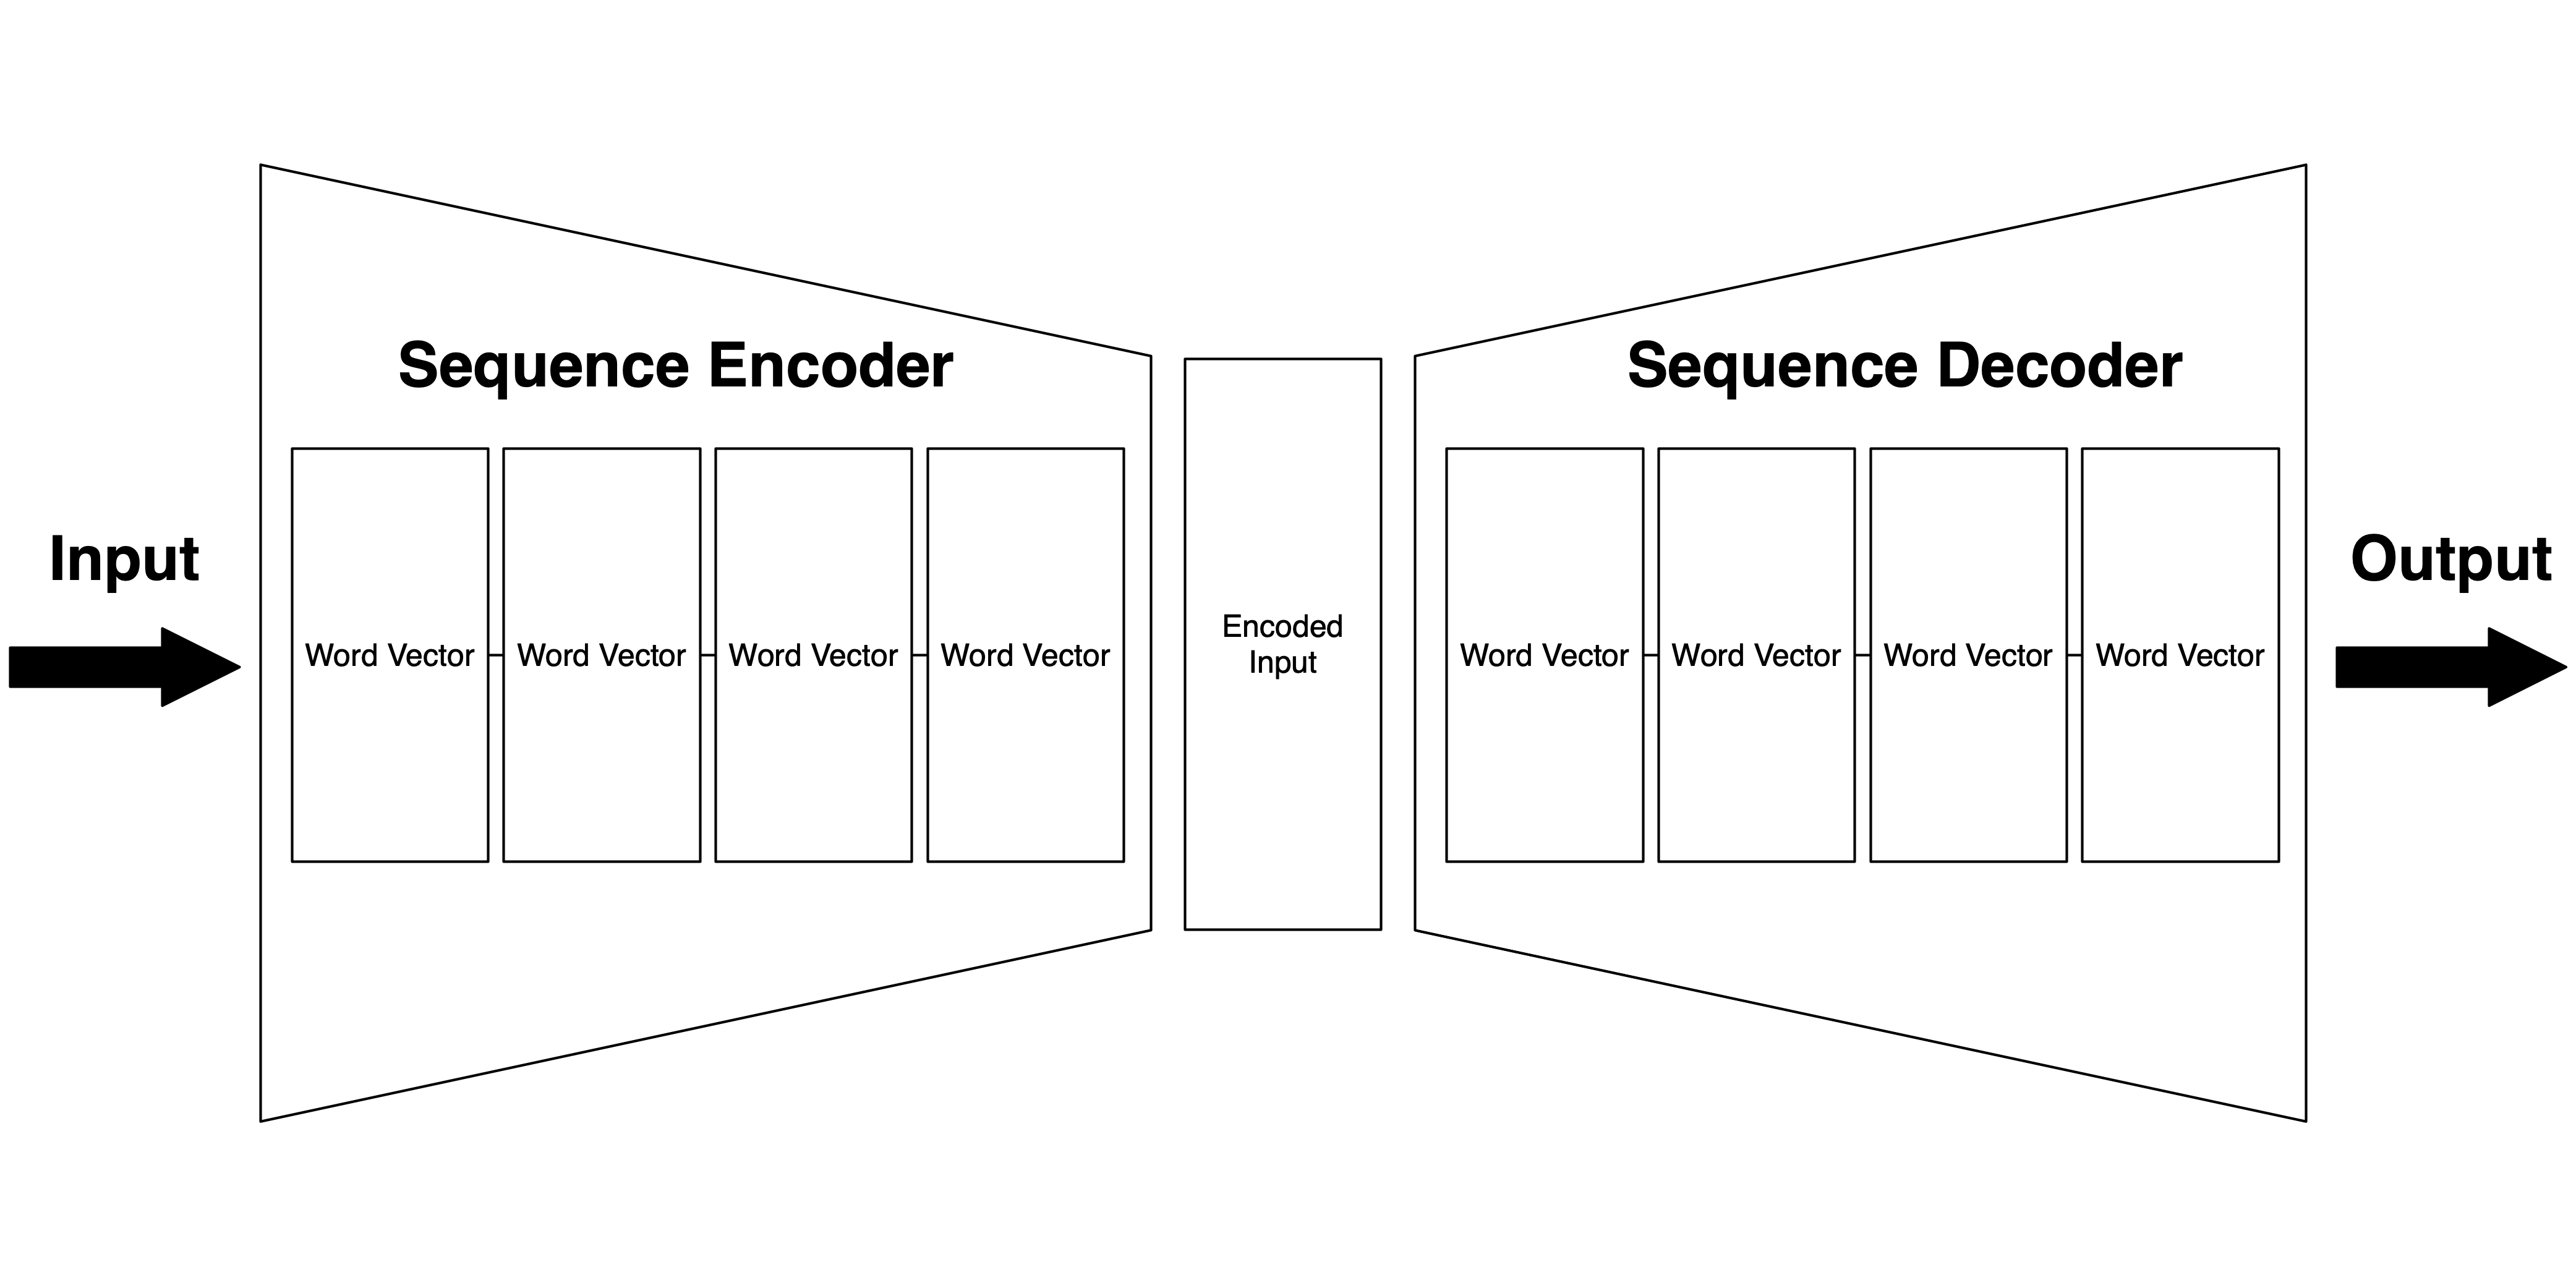
\includegraphics[width=\textwidth,keepaspectratio=true]{fig_supervised_chabots}
    \caption{Illustrative representation of a Sequence to Sequence architecture.}
    \label{fig:fig_supervised_chabots}
\end{figure}

\subsection{Adversarial Learning}
\label{chatbot:adversarial}
\gls{al} has driven attention thanks to Computer Vision \gls{gan} \autocite{paper:Karras2019stylegan2} by proving that it is possible to generate realistic human face \autocite{website:person_does_not_exist}. In the chatbots context, it can be extrapolated into a futuristic version of the Turing Test \ref{chatbot:history}, where machines are confronting themselves instead of humans. The concept implies the use of a training dataset containing human conversations, and compare them against the generated answer; the discriminator will then judge which is from a human and which is from an algorithm. Note that adversarial methods such as \gls{gan} are working well because of the nature of the data it plays with; indeed, pixels can be deeply noised, but words cannot be due to their discrete nature. See Figure ~\ref{fig:fig_adversarial_chatbots} 

\begin{figure}[H]
    \centering
    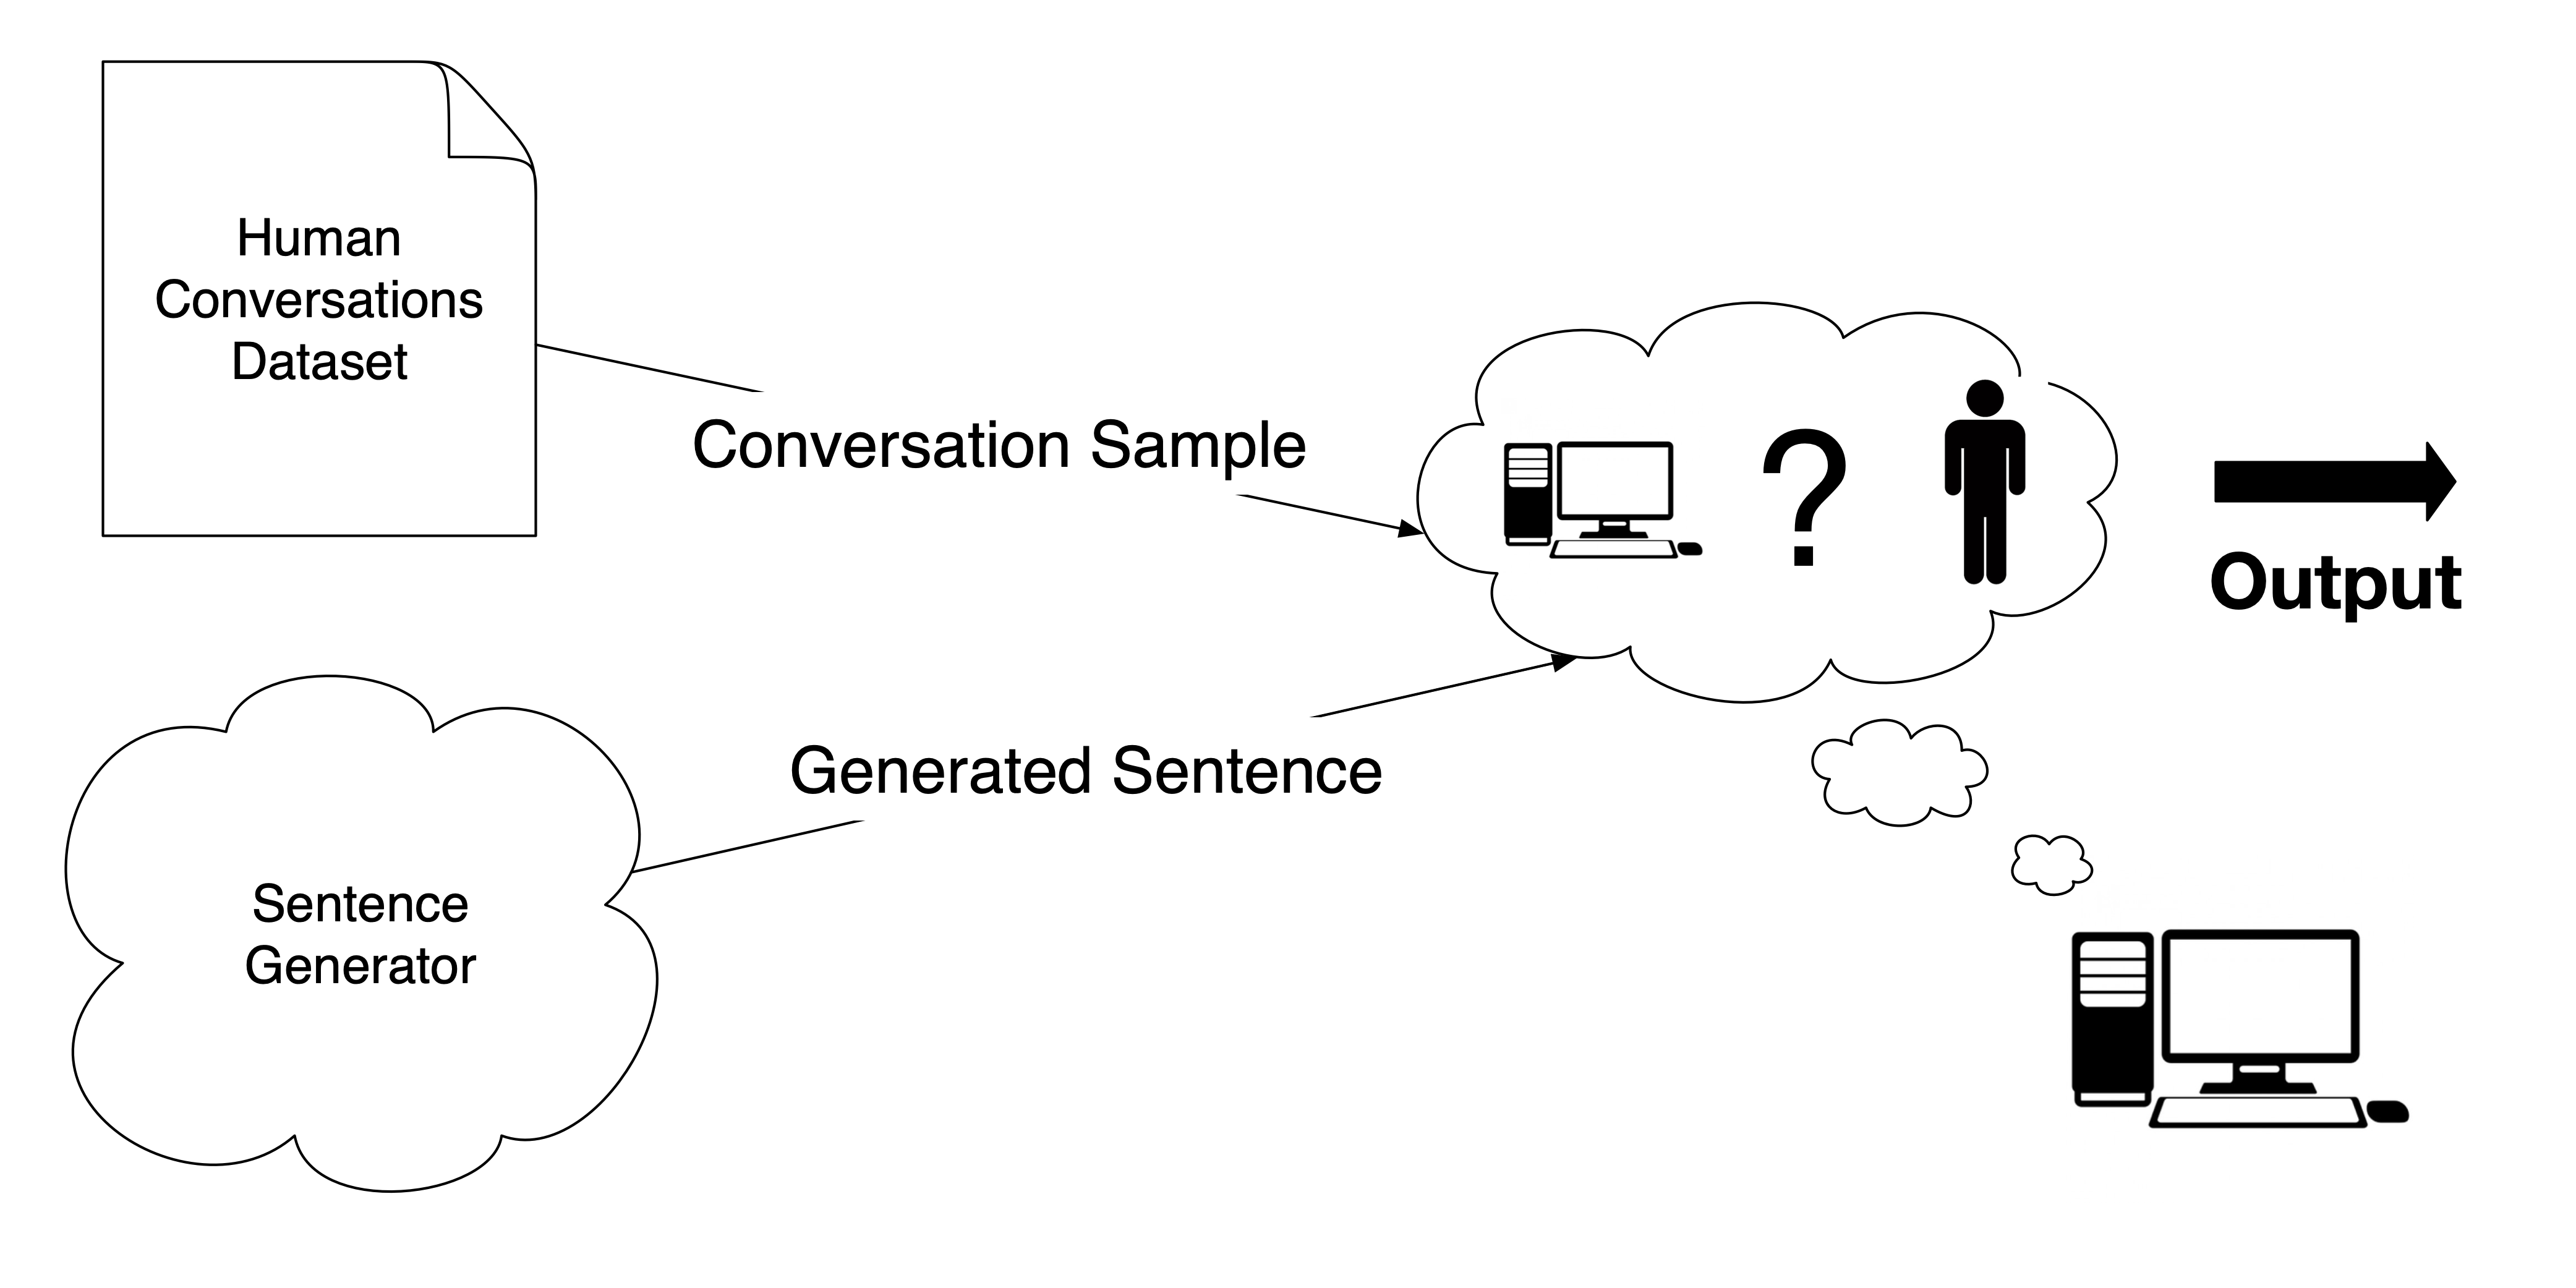
\includegraphics[width=\textwidth,keepaspectratio=true]{fig_adversarial_chatbots}
    \caption{Illustrative representation of an adversarial architecture in a chatbot context.}
    \label{fig:fig_adversarial_chatbots}
\end{figure}

\subsection{Pre-trained Language Models}
Language Models are currently the most recent and the most promising models due to their ability to model language itself instead of conversations and then tune the outputs as a chatbot would. It can been seen as semi-supervised learning, as it uses \gls{ul} for training and supervised learning \ref{chatbot:supervised} for fine-tuning \ref{chatbot:finetuning}. We will dive into \gls{lm} in the \gls{nlp} chapter \ref{nlp-lm}.

\subsection{Model Fine-Tuning}
\label{chatbot:finetuning}
With the specificity of \gls{model-ft}, {lm} as it provides the tools to build chatbots based on the ground of the language itself and then customize the model into a specific manner by fine-tuning it on a dataset fitting the domain required by the chatbots. Indeed, it is relatively easy to fine-tune a \gls{qa} dataset to a \gls{lm}, making the model able to answer questions instead of descriptively filling sentences. The main downside to those models is the large memory size required to run them. However, due to their nature, they are trained once and then fine-tuned. Note that training requires an enormous amount of computational power. E.g, The largest form of BERT \autocite{paper:devlin-etal-2019-bert} was trained on 16 TPUs for 4 days. Fine-tuning, on the other hand, scales down to few hours on a single TPU, which makes it relatively scalable to new domains. See Figure ~\ref{fig:fig_finetunedmodel_chatbots} 

\begin{figure}[H]
    \centering
    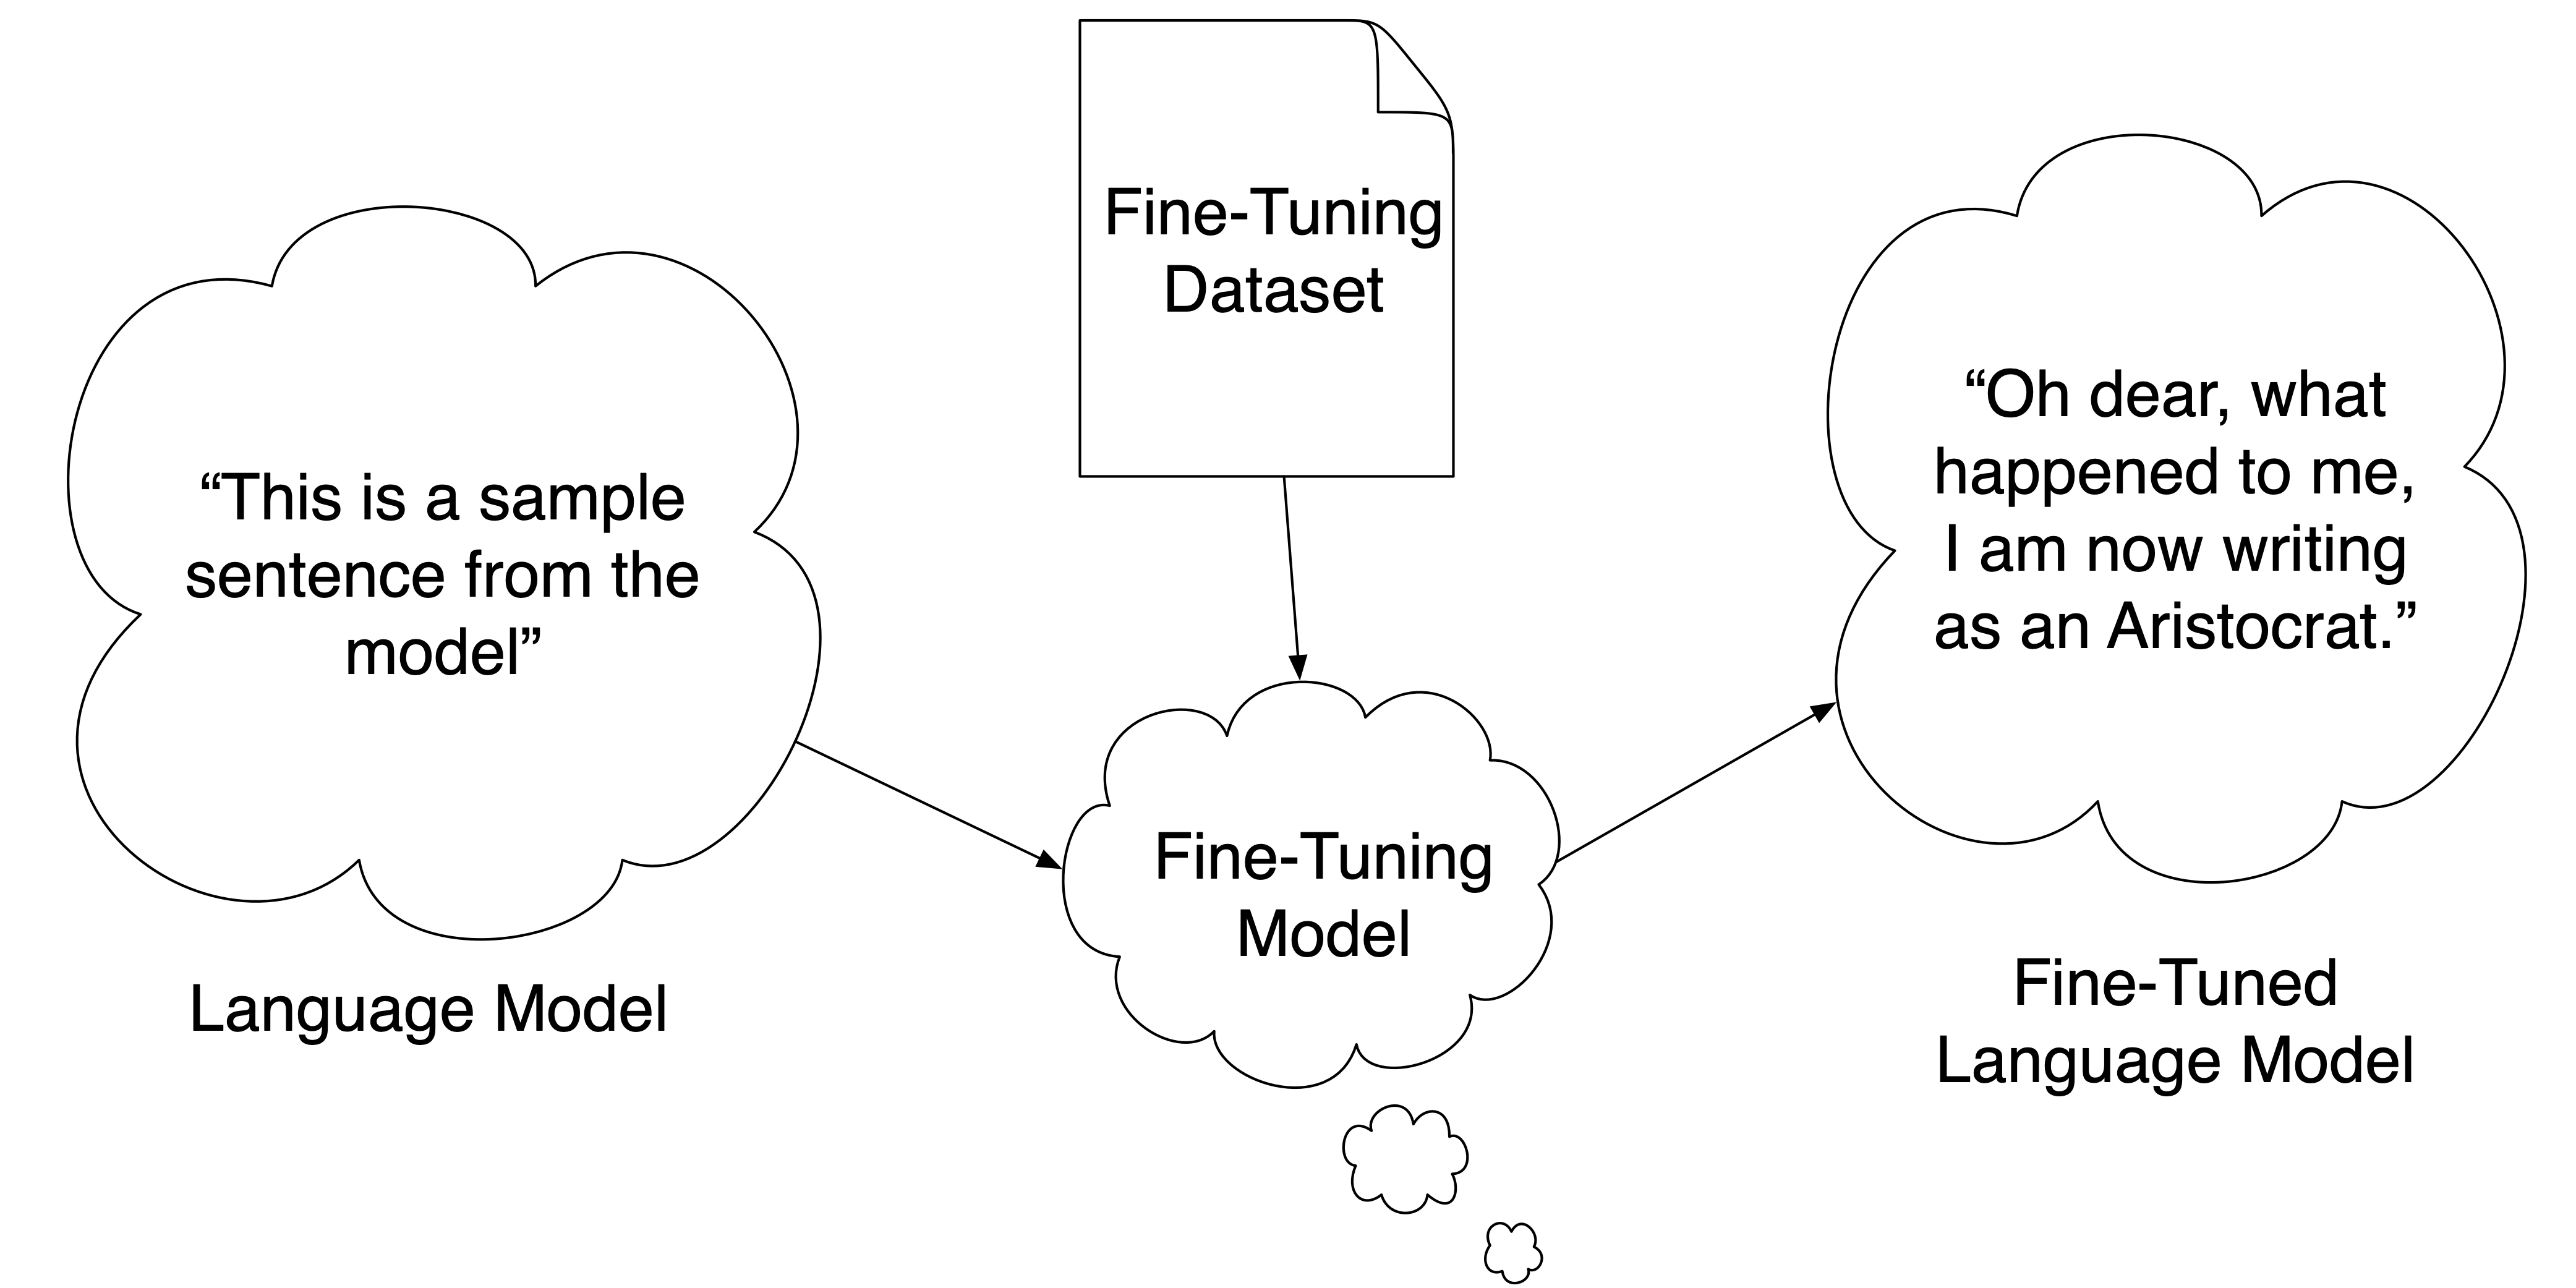
\includegraphics[width=\textwidth,keepaspectratio=true]{fig_finetunedmodel_chatbots}
    \caption{Illustrative representation of fine-tuning in a chatbot context.}
    \label{fig:fig_finetunedmodel_chatbots}
\end{figure}

\subsection{Reinforcement Learning}
\gls{rl} is proven to be very powerful by the latest research made by \textit{Open-AI} with its DOTA2 bot or \textit{Google's Deepmind} with AlphaZero, so we believe that it is worth mentioning it. However, this type of learning requires a finite state similar to a \gls{mdp}, which matches game cases but not conversations, and impacting by this means the motivation to export the technique to \gls{nlp}. Indeed, this methodology requires that all information required for the next step are wrapped into a single state to predict it, which makes it hard to use the dialogue case. For now, \gls{nlp} research does not provide a conclusion as if, with billions of simulations, \gls{rl} Chatbots could reach comparative results to Generative Chatbots \ref{chatbot:generative}.

\section{Grounded Chatbots}
\label{chatbot:grounded}
Falling in a particularly rare research field of \gls{ml} and \gls{nlp}, \gls{gl} can be seen as the future of \gls{mu} and \gls{mr}. In a chatbot context, the goal is to simulate, based on the Grounded Theory from the social sciences, how humans are using inductive reasoning to create conversations with unstructured knowledge. The idea is to give the ability to the bot, for any given input, to gather information from any data sources and provide an inductive output. E.g., Combining Knowledge Bases with weather forecaster. Second e.g., For example, for the given input: \say{What is the color in autumn of a leaf in Switzerland?}, 1) the bot would have first to identify the context keywords (color, leaf, autumn, switzerland), 2) the bot would select where to gather the information, 3) the would investigate the Wikidata Knowledge Base, Wikipedia, and The Weather Channel API, 4) the bot would formulate an answer based on the information it gathered. ~\ref{fig:fig_grounded_chatbots}

\begin{figure}[H]
    \centering
    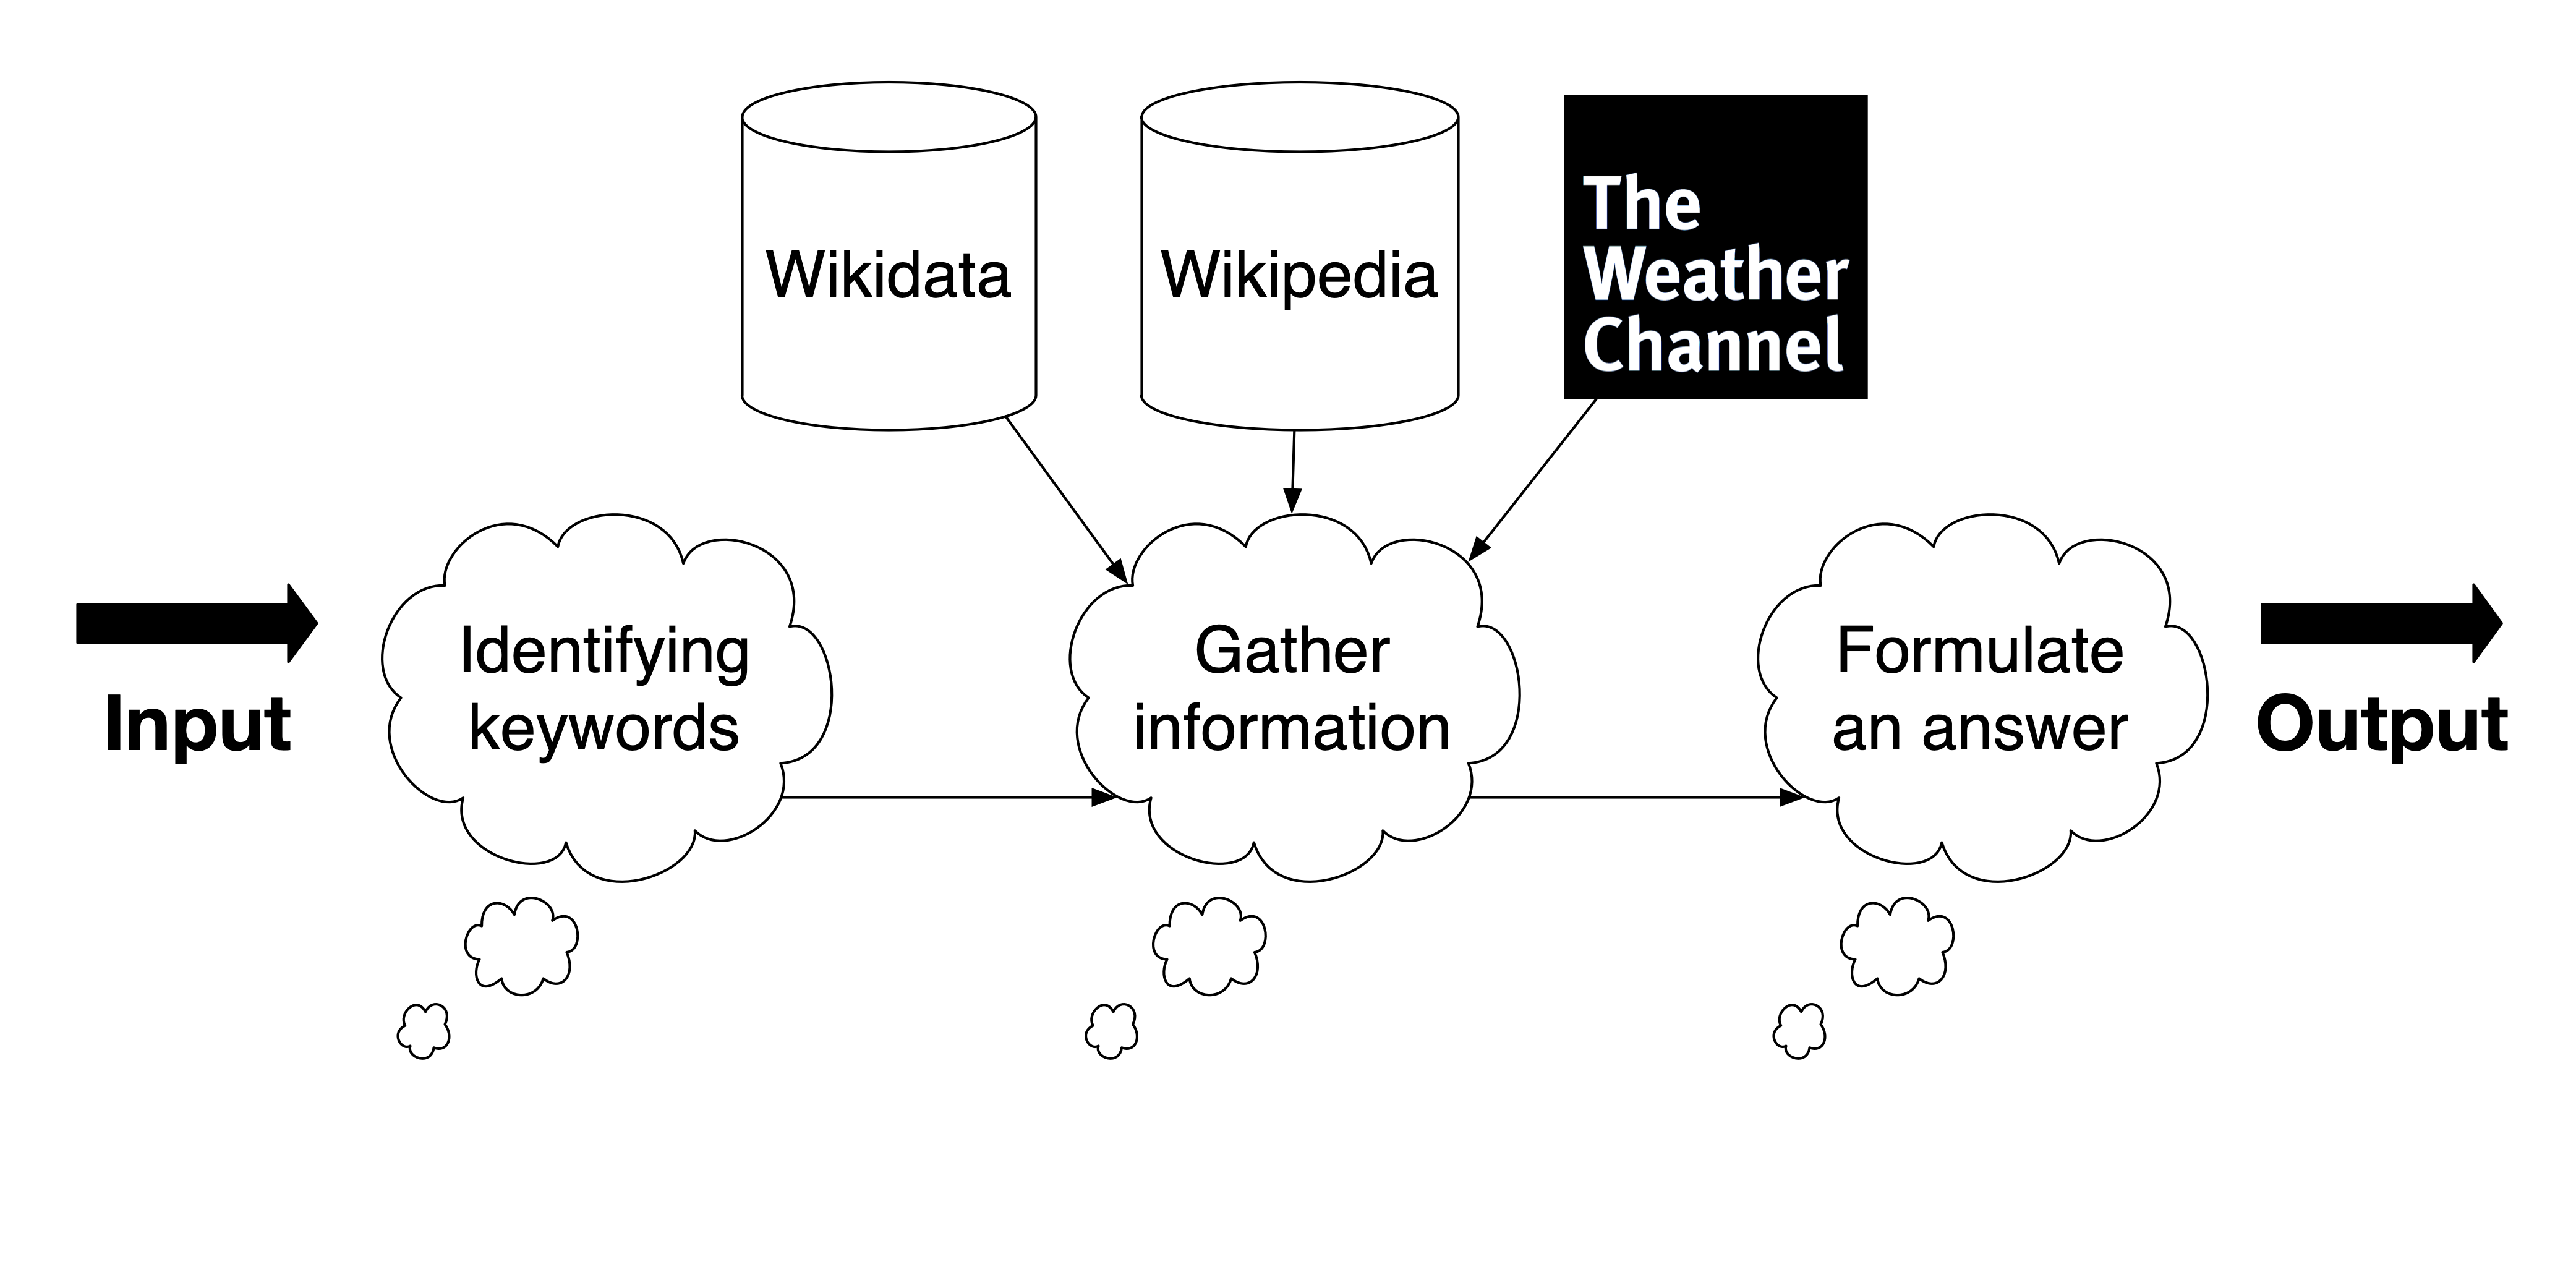
\includegraphics[width=\textwidth,keepaspectratio=true]{fig_grounded_chatbots}
    \caption{Illustrative representation of a grounded chatbot.}
    \label{fig:fig_grounded_chatbots}
\end{figure}

\section{Question-Answering Chatbots}
\gls{qa} is a prevalent task for chatbots; indeed, they are widely used for questioning tasks in either Single or \gls{open-domain}, Open or \gls{closed-ended}, Single or \gls{mh} with applications such as FAQs, Supports, help to find the meaning of life, and so on. Due to the broadness of the field, no defined methodology has been generalized; instead, it uses either one or multiple techniques described in the previous sections. It is interesting to note that the field of \gls{qa} is raising a lot of interest in \gls{nlp} research lately, and the benchmarking game of creating the new baselines, with increasingly complex datasets, is still in progress. In this section, we will overview some recent baselines.

\paragraph{Fine-Tunning Language Models} Large \gls{lm} such as BERT \autocite{paper:devlin-etal-2019-bert} or GPT-2 \autocite{papers:gpt2} are often fine-tuned on \gls{qa} datasets similar to SQUAD 2.0 \autocite{paper:rajpurkar-etal-2018-know} which are particularly tricky, even for humans.

\paragraph{Querying Models} Based on \gls{qa} datasets, a model is trained to fill structured templates.  The generated output is a structured query for a particular querying language such as SPARQL for Wikidata. 

\paragraph{Retrieval} A popular approach in the industry is to use tools such as Elasticsearch for indexing and additional tools using \gls{ml} heuristics to perform the queries.

\clearpage
\section{Common Chatbot Features Overview}
In this section, we are non-exhaustively naming a few recurring features appearing during our targeted research.

\subsection{Context}
Humans are intuitively and extensively relying on the context for conversational purposes, chatbots relying on dialogue as part of their task, requires the capacity to hold context. On a side note, one-way style dialogues such as commands or none-nested questions do not need to hold context to perform well.

\paragraph{Short term context} Implying the ability for the bot to hold context for at least the current conversation, e.g., few keywords or on-the-fly \gls{model-ft}.

\paragraph{Long term context} Often, chatbots would use user-profiles as part of their architecture to remember information such as the favorite pizza flavor of a client. 

\subsection{Proactivity}
Simulating personalized interest as a human would do is not new to chatbots, as it has been proven by becoming a standard in marketing and customer support chatbots. Messages such as \say{Hey, you are on our web store for a while, can I help you?}, are carrying a sense of proactivity; however, beyond asking general pre-made questions, limitations are clear, and not much progress has been made yet in the field. Indeed, human-like proactive chatbots imply algorithms capable of initiating conversations by initiating a dialogue or asking information in a meaningful manner based on the long and short term context.

\subsection{Narrow vs General Chatbots Scope}
Beyond the three main categories \ref{chatbot:main-cats} identified during the study, in general, chatbots can additionally be classified within a scope starting at Narrow Chatbots up to General Chatbots. To position them, we defined a two axes classification using Tasks and Knowledge as represented on Table \ref{tab:agi-ani}.

\paragraph{Tasks Axis}
To name a few examples of task-oriented Chatbots: Talk, \gls{faq}, Customer Support, or Ordering.

\paragraph{Knowledge Axis}
Non-exhaustively, as follows, a few knowledge-centric examples for chatbots: Health, Weather, or Customer Service.

\paragraph{Narrow Chatbots}
Narrow chatbots are limited by the range of tasks they can accomplish and the knowledge they can use. By design, they are very good at a particular task for a particular knowledge requirement.

\paragraph{General Chatbots}
They are neither limited by the range of tasks they can accomplish or the knowledge they can use. However, they often have an average performance for any task or knowledge. We go in more details at section \ref{chatbot:general}.


\newcommand\MyBox[2]{
  \fbox{\lower0.75cm
    \vbox to 2cm{\vfil
      \hbox to 6cm{\hfil\parbox{5cm}{#1\\#2}\hfil}
      \vfil}
  }
}

\setlength\tabcolsep{0pt}
\begin{table}[H]
\centering
\begin{tabular}{c >{\bfseries}r @{\hspace{0.7em}}c @{\hspace{0.4em}}c @{\hspace{0.7em}}l}
  \multirow{6}{*}{\rotatebox{90}{\parbox{2.4em}{\bfseries\centering Tasks}}} 
  & & \MyBox{Expert in a specific Field}{Expert at all Tasks} & \MyBox{\textbf{General Chatbots}\\Expert in all Fields}{Expert at all Tasks} \\[2.4em]
  & & \MyBox{\textbf{Narrow Chatbots}\\Expert in a specific Field}{Expert at specific Task} & \MyBox{Expert in all Fields}{Expert at specific Task} \\[2.4em]
  & & \multicolumn{2}{c}{\bfseries Knowledge} & \\
\end{tabular}
\caption{This table represents categories in Narrow and General Chatbots in a Tasks versus Knowledge format.}
\label{tab:agi-ani}
\end{table}


\subsection{General Chatbots}
\label{chatbot:general}
As research progress in the \gls{nlp} field, chatbots are improving as an effort to perform simultaneously well in various tasks and multi-knowledge bases. As a contemporary goal, in addition to any chatbot related tasks and broad knowledge expertise, General Chatbots must not be limited to their current capabilities, but on the contrary, be able to learn new tasks and subjects continuously. As far as we as this study went, we could not find \gls{sota} general chatbots as defined. However, companies like \textit{Amazon} are selling to a large public a feel to general chatbots with Alexa. Indeed, apart from ordering goodies from \textit{Amazon} and roughly conversing with Alexa, users can command their smart homes, use it as a personal assistant, or even program \textit{skills} to perform custom actions.

\clearpage
\section{Chatbots Cartography}
As a result of this chapter, we created a chart on Figure ~\ref{fig:fig_chatbot_cartography} representing the current state of chatbots from our point of view. Note that a particular use-case could be in multiple leafs.

\begin{figure}[H]
    \centering
    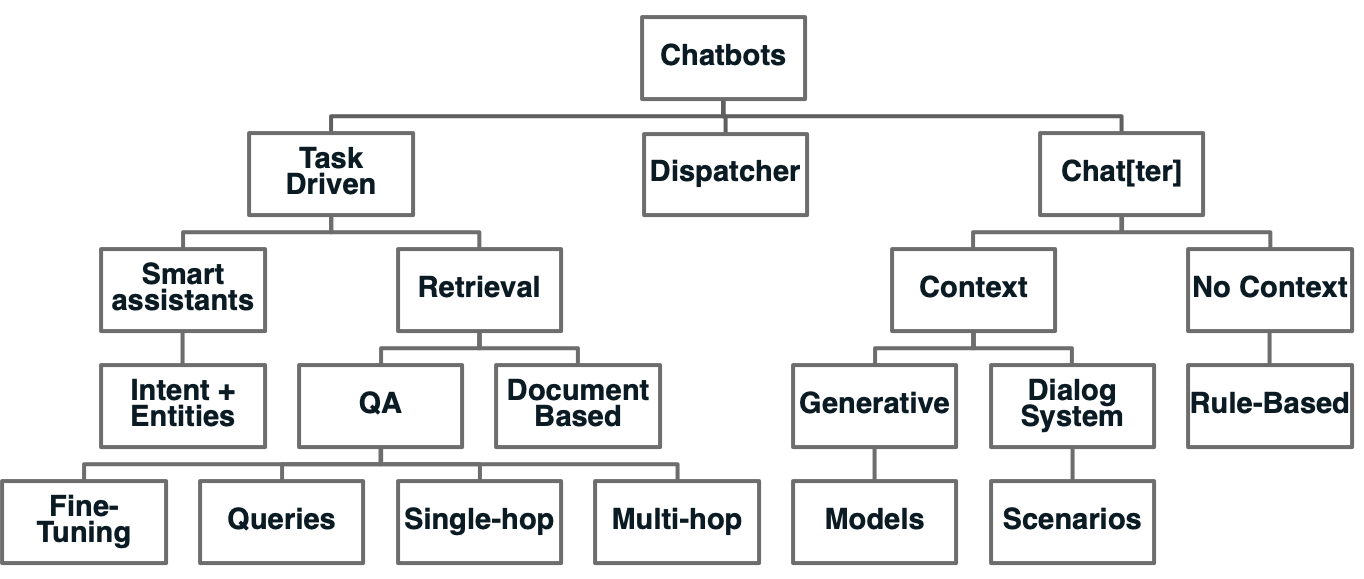
\includegraphics[width=\textwidth,keepaspectratio=true]{fig_chatbot_cartography}
    \caption{Represents the chatbots cartography as conclusion to the chatbot state-of-the-art chapter.}
    \label{fig:fig_chatbot_cartography}
\end{figure}





